% Per-Season Brier Score Comparison (2015--2024)
% Complements: tab:per-season-top3 / tab:oos-record
% Line chart showing calibration consistency across 10 seasons

\begin{figure}[htbp]
\centering
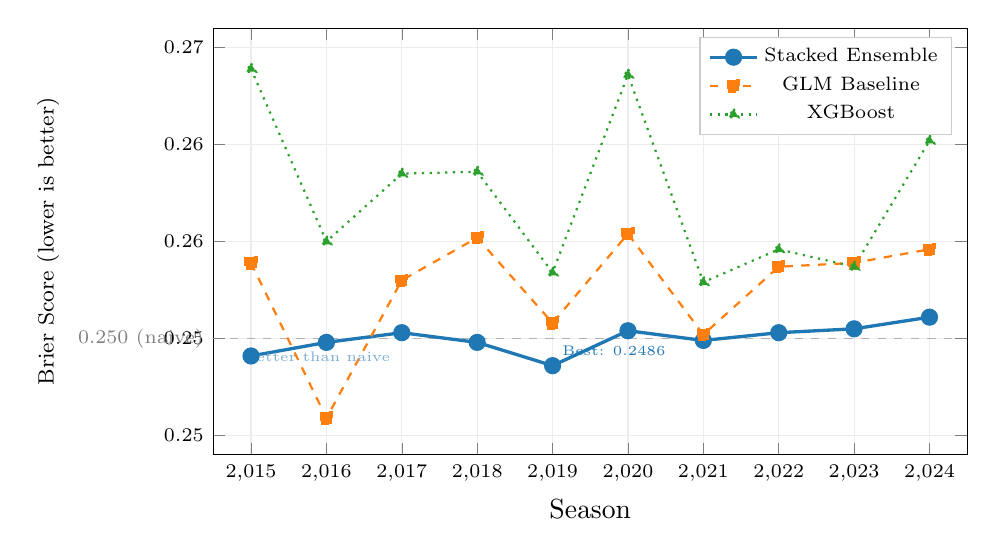
\begin{tikzpicture}
\definecolor{accent}{RGB}{31,119,180}
\definecolor{accentOrange}{RGB}{255,127,14}
\definecolor{accentGreen}{RGB}{44,160,44}

\begin{axis}[
  width=0.92\textwidth,
  height=7cm,
  xlabel={Season},
  ylabel={Brier Score (lower is better)},
  ylabel style={font=\footnotesize},
  xmin=2014.5, xmax=2024.5,
  ymin=0.244, ymax=0.266,
  xtick={2015,2016,...,2024},
  xticklabel style={font=\scriptsize},
  ytick={0.245,0.250,0.255,0.260,0.265},
  yticklabel style={font=\scriptsize},
  grid=major,
  grid style={gray!15},
  legend style={at={(0.98,0.98)}, anchor=north east, font=\scriptsize, draw=gray!40},
  % Highlight the 0.250 baseline
  extra y ticks={0.250},
  extra y tick labels={0.250 (naive)},
  extra y tick style={grid style={black!30, dashed}, tick label style={font=\tiny, color=black!50}},
]

% Stack (ensemble) line
\addplot[accent, very thick, mark=*, mark size=2.5pt] coordinates {
  (2015, 0.2491) (2016, 0.2498) (2017, 0.2503) (2018, 0.2498)
  (2019, 0.2486) (2020, 0.2504) (2021, 0.2499) (2022, 0.2503)
  (2023, 0.2505) (2024, 0.2511)
};
\addlegendentry{Stacked Ensemble}

% GLM line
\addplot[accentOrange, thick, mark=square*, mark size=2pt, dashed] coordinates {
  (2015, 0.2539) (2016, 0.2459) (2017, 0.2530) (2018, 0.2552)
  (2019, 0.2508) (2020, 0.2554) (2021, 0.2502) (2022, 0.2537)
  (2023, 0.2539) (2024, 0.2546)
};
\addlegendentry{GLM Baseline}

% XGBoost line
\addplot[accentGreen, thick, mark=triangle*, mark size=2pt, dotted] coordinates {
  (2015, 0.2639) (2016, 0.2550) (2017, 0.2585) (2018, 0.2586)
  (2019, 0.2534) (2020, 0.2636) (2021, 0.2529) (2022, 0.2546)
  (2023, 0.2537) (2024, 0.2602)
};
\addlegendentry{XGBoost}

% Annotation: ensemble consistency
\node[font=\tiny, text=accent, anchor=south west, align=left] at (axis cs:2019,0.2486)
  {Best: 0.2486};

% Shade the region where ensemble beats naive
\addplot[accent!8, forget plot, draw=none] coordinates {
  (2014.5, 0.244) (2014.5, 0.250) (2024.5, 0.250) (2024.5, 0.244)
} \closedcycle;

\node[font=\tiny, text=accent!60, anchor=north west] at (axis cs:2014.8,0.2498)
  {better than naive};

\end{axis}
\end{tikzpicture}
\caption[Per-season Brier scores]{Per-season Brier score comparison (2015--2024). The stacked ensemble (blue) achieves consistently lower Brier scores than both GLM baseline (orange) and XGBoost (green), with remarkably low variance across 10 seasons ($\sigma = 0.0007$). All ensemble seasons beat the 0.250 naive baseline. XGBoost shows higher year-to-year volatility, particularly in 2015 and 2020.}
\label{fig:per-season-brier-chart}
\end{figure}
